\documentclass[12pt]{article}

%%% Packages %%%

\usepackage[utf8]{inputenc}
\usepackage{titlesec}
\usepackage{graphicx}
\usepackage[margin=1in]{geometry}

%%% Styles %%%

\titleformat{\chapter}{\normalfont\huge}{\thechapter.}{20pt}{\huge\it}

\titleformat{\paragraph}
{\normalfont\normalsize\bfseries}{\theparagraph}{1em}{}
\titlespacing*{\paragraph}
{0pt}{3.25ex plus 1ex minus .2ex}{1.5ex plus .2ex}

\bibliographystyle{abbrv}

%%% Document information %%%

\title{
	{
	
\includegraphics[width=0.7\linewidth]{logo-fib.png}	
	\vspace{1cm}
	\textbf{\\Project planning} \\
	\large New real-time GNSS algorithms for detection and measurement of potential geoeffective stellar flares}
\author{\textbf{Author}\\
	David Moreno Borr\`as
	\\ \\
	\textbf{Supervisor}\\
	 Manuel Hernández-Pajares}
\date{\today}
}


%%%%%%%%%%%%%%%%%%%%%%%%%%%%%%%%%%%
%%%%%%% Start of document %%%%%%%%%
%%%%%%%%%%%%%%%%%%%%%%%%%%%%%%%%%%%

\begin{document}
	
\pagenumbering{arabic}
\clearpage
\maketitle
\thispagestyle{empty}
\clearpage


\tableofcontents
\thispagestyle{empty}
\clearpage

%%%%%%%%%%%%%%%%%%%%%%%%%%%%%%
%%%%%%% Planning and scheduling %%%%%%%%%
%%%%%%%%%%%%%%%%%%%%%%%%%%%%%%

\section{Planning and scheduling}

The aim of this document is to present the tasks and stages of the project and how are they going to be planned and scheduled so the project meets its objectives within the given deadlines.

Because we rely on some stages of the project to work before we begin to tackle others, this planning might be updated as the project progresses, perhaps because a part took longer to develop than expected or (luckily) less.

%%%%%%%%%%%%%%%%%%%%%%%%%%%%%%%%%%%%%
%%%%%%% Task description %%%%%%%%
%%%%%%%%%%%%%%%%%%%%%%%%%%%%%%%%%%%%%

\section{Task description}

In this section a description of each task is presented in a similar order to that which will be seen later in the planning section.

\paragraph{Introduction to the problem}

Study past research papers related to the problem to gain some background on the project, this includes the following topics:

\begin{itemize}
  \item The use of GNSS data as a solar flare meter. Some research papers about this topic were discussed in the State of the Art section, most of them written by the director, Manuel Hernández-Pajares. \cite{hernandez2012gnss}
  \item Solar and stellar bursts and their effect on Earth’s ionosphere. The aforementioned papers give a brief introduction to the topic, although others can be found that cover the topic with more depth. \cite{mitra1974ionospheric}
\end{itemize}

\paragraph{GEP}

The GEP course is done early in the project to help with the documentation of the thesis, understanding the scope and context of the project, and its planning. Its different stages are:

\begin{itemize}
	\item Context and Scope of the project
	\item Project planning
	\item Budget and sustainability
\end{itemize}

This also involves a final deliverable that includes the previously listed parts but taking into consideration the feedback of the professors of the course.

Finally, an oral presentation will be done describing the work done during this course, which will also be a starting point of the final presentation of the thesis.

\paragraph{Feasibility of the detection of flares from far-away stars}

Before developing the algorithms to be able to perform this without knowing the source of the flare, a study should be done with the already existing algorithms. This is one of the most challenging problems of the project as it is not clear yet if this is possible.

To do this, we will use open-source data from missions like Swift or Fermi (satellites that are able to detect flares or burst) and see if there is any correlation between that data and the results given by the algorithms that detect solar flares.

\paragraph{Detection of solar flares with no information about the location of the Sun}

This task will be done in parallel to the previous one. The current algorithms are able to, knowing the position of the Sun, study if any flares have had an effect on the ionosphere, detectable by the satellites belonging to GNSS. 

We aim to do the same, but assuming we don’t have any information about the position of the Sun relative to the Earth. This is an important task for the project, because it will be necessary when expanding it to far-away stars, of which we ignore the location.

\paragraph{Detection of stellar flares in real-time}

If the previous systems work, instead of studying flares using past GNSS data and checking that the results match detections by satellites like Swift or Fermi, we will use the latest available data to detect them in real-time, without knowing the location of the ionizing source. For this to work the detection of far-away stars using this system and the detection of solar flares without knowing the location of the Sun have to work properly.

\paragraph{Writing the report}

This task will be done in parallel to the rest. As we perform the other tasks a memory of the project will be written giving a detailed explanation of all the phases, the methodology and development of the solutions, problems or obstacles that might have appeared, and the final results of each of them. 

\paragraph{Final presentation}

The final task, once the report of the project is finished, is to prepare an oral presentation for the defense of the thesis. This will try to cover all the progress of the work done during the last months as concisely as possible, presenting the results, obstacles that may have appeared and solutions presented for the problems.

%%%%%%%%%%%%%%%%%%%%%%%%%%%%%%%%
%%%%%%%%%% Time table %%%%%%%%%%
%%%%%%%%%%%%%%%%%%%%%%%%%%%%%%%%
\section{Time table}

Table 1 shows the estimation of the amount of hours that will have to be dedicated for the completion of each task. The expected amount of dedicated hours to the project is 18 ECTS x 30h/ECTS = 540 hours, of which 3x30 = 90 hours are dedicated to the GEP course.

\begin{table}[h!]
	\centering
	\begin{tabular}{||c c||} 
		\hline
		Task & Dedication Time (hours) \\ [0.5ex] 
		\hline\hline
		Introduction & 20  \\ 
		\hline
		GEP & 90  \\
		\hline
		Study of flares from far-away stars & 120 \\
		\hline
		Detection of solar flares & 120  \\
		\hline
		Detection in real-time & 100  \\ 
		\hline
		Writing report & 90  \\ 
		\hline
		Final presentation & 4 \\
		\hline\hline
		Total & 544  \\
		\hline
	\end{tabular}
	\caption{Dedication time to each of the tasks}
	\label{table:1}
\end{table}

Taking into consideration the project will span 14 weeks, a weekly dedication of 34 hours is possible for the project planning to work as scheduled.

%%%%%%%%%%%%%%%%%%%%%%%%%%%%%%%%
%%%%%%%%%% Scheduling %%%%%%%%%%
%%%%%%%%%%%%%%%%%%%%%%%%%%%%%%%%
\section{Scheduling: Gantt chart}

Having started mid-February, the development of the project will span between 4 or 5 months as the oral presentations are scheduled for the first week of July. 

The report should be handed in one week prior to the lectures, so for the planning, our objective is to finish the project a week before: Friday, 21th of June, so that there is enough time to revise it and make any convenient changes.

To visually represent the schedule of the planning, a Gantt chart is shown below in Figure 1. This chart has been generated using the online tool teamgantt.com: 

\vspace{0.25cm}

\begin{figure}[ht]
	\centering	
	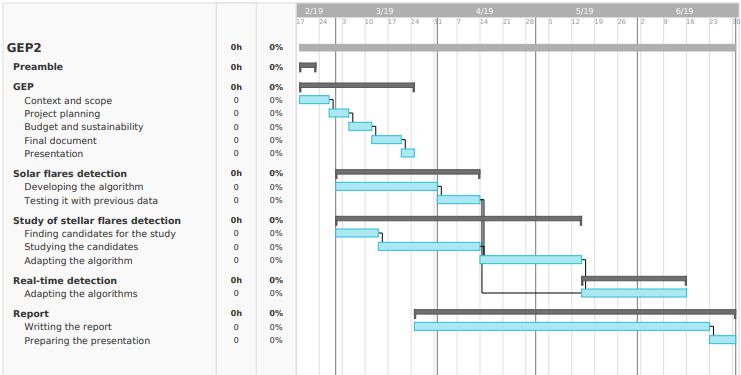
\includegraphics[width=0.9\linewidth]{gantt.png}
	\caption{Gantt chart with the planning of the project }
\end{figure}
	

%%%%%%%%%%%%%%%%%%%%%%%%%%%%%%%%
%%%%%%%%%% Action plan %%%%%%%%%%
%%%%%%%%%%%%%%%%%%%%%%%%%%%%%%%%
\section{Action plan}

Our idea is to work in the presented order as planned in the the previous sections, some tasks depend on previous ones to be finished to continue, and others are going to be done in parallel, like writing the report. 

Time is limited and many problems might appear that will force us to reschedule the project planning, some of which could be:

\paragraph{Understanding of the problem}

The problem has a considerable physics background that I, as a Computer Science student, lack the knowledge to completely understand it. Although a basic knowledge in the field will suffice for developing the algorithms, not having a background in physics might lead to confusion at some point.

\paragraph{Unfeasibility of the solution}

The problem that we want to solve is clear: detecting stellar flares from far-away stars. This has been studied for some cases \cite{martinez2016first}, concluding that we face the possibility that the proposed solution is not totally feasible due to the nature of the problem: flares from far-away stars will not have an impact on the ionosphere as noticeable as the one from the sun, so it may be difficult, or even impossible, for them to be detected in some cases.

\paragraph{Interferences with the Sun}

With the Sun, only the daylight hemisphere is studied for the detection of flares using GPS data (it is the only one flares' effects can reach)

In our case we don’t have a fixed source, but rather aim to find it. Flares could be having an effect on any part of the ionosphere so it may not be possible to study their effect on the daylight hemisphere because of the Sun’s (presumably) higher effect on it. 

Because of this factor we might have to focus only on the night hemisphere and we would be missing on possible flares.

\paragraph{Understanding previous algorithms}

It is often difficult to understand code that has not been written by oneself, let alone understanding complex algorithms without any previous knowledge. This could be another possible obstacle, as the study of the previously developed algorithms will play an important role in the development of ours.

\paragraph{Bugs}

As we will be writing code it is clearly possible that we face problems with bugs that may appear in the process.

\paragraph{Computational power}

Taking into consideration we may be dealing with large volumes of data, its processing may be another challenge for the project, we will have to find efficient ways to do so and think about which strategies will work best in our algorithms.  \\ 

Despite this possible obstacles, with the previous planning and a weekly dedication of 34 hours we think the project is feasible.

%%%%%%%%%%%%%%%%%%%%%%%%%%%%
%%%%%%% References %%%%%%%%%
%%%%%%%%%%%%%%%%%%%%%%%%%%%%

\newpage

\bibliography{references}

\end{document}